\chapter{Proposta de Trabalho}\label{chap:proposta}

%--------------------------------------------------------------------------------
\section{Considerações Iniciais}

A proposta deste trabalho gira em torno do conceito de \emph{projeções multidimensionais coordenadas entre itens e atributos}. 

A metodologia proposta por este trabalho é inspirada em uma combinação entre as projeções de atributos de~\cite{Yang2004} e às visões duplamente coordenadas entre itens e atributos de~\cite{Turkay2011}. 

O processo de projeção dos atributos inicia pela criação de uma matriz de distâncias que busca capturar os relacionamentos entre as dimensões. Em seguida, com base nessa matriz, aplica-se um método semelhante a MDS para posicionar os atributos em um plano bidimensional. Diferentemente de \cite{Yang2004}, aqui as dimensões não serão representadas por glifos, mas sim por pontos. Apesar de glifos serem capazes de fornecer informações adicionais sobre os dados, no caso de projeções eles acentuam o problema de sobreposição de elementos.

A etapa de coordenação entre visões dos itens e atributos será realizada 


%--------------------------------------------------------------------------------
\section{Objetivos}

% Falo como vou resolver as limitações levantadas e assim cito as contribuições esperadas do trabalho:

% 1. Acompanhamento do estado da arte dos trabalhos em estatística
% 2. Mecanismos intuitivos para seleção e combinação
% 3. Um novo mecanismo que permite a transformação do espaço de atributos
% 4. Uma única metáfora visual (projeções)

Dentro do contexto apresentado anteriormente, o seguinte parágrafo representa a declaração dos objetivos deste trabalho de mestrado:

\begin{quote}
    \emph{``Este projeto de mestrado tem como objetivo desenvolver mecanismos interativos sobre projeções multidimensionais coordenadas entre atributos e itens que auxiliem o usuário na tarefa de redução de dimensionalidade. Os mecanismos devem permitir tanto a seleção quanto a combinação de atributos. Caso os resultados não reflitam o conhecimento do usuário, este poderá manipular as projeções para transformar o espaço de atributos de modo a criar um modelo mais representativo.''}
\end{quote}

As seguir apresenta-se os passos necessários para atingir esses objetivos.

%--------------------------------------------------------------------------------
\section{Metodologia}

A metodologia proposta por este trabalho é ilustrada pela Figura~\ref{fig:met}. O processo inicia pelo cálculo da similaridade entre as dimensões. Com base neste cálculo, cria-se uma matriz de distâncias entre os atributos que é utilizada para projetá-los em um espaço bidimensional.   

inicia pela escolha de uma medida para o cálculo da similaridade entre pares de dimensões. Com base nessas distâncias projeta-se as dimensões utilizando alguma técnica de projeção multidimensional, como MDS. Neste ponto permite-se que o usuário utilize os mecanismos interativos de redução de dimensionalidade e de transformação do espaço de atributos. Ele pode, por exemplo, construir um espaço dimensional reduzido que é prontamente apresentado em visualizações coordenadas. Finalmente, se o resultado obtido não for satisfatório, o usuário pode iniciar novamente o ciclo partindo do novo espaço dimensional construído, ou pode realizar novas manipulações sobre os dados.

% Melhorar este parágrafo e colocar uma figura para ilustrar o processo.

\begin{figure}[h!]
    \centering
    \begin{subfigure}[b]{0.5\textwidth}
        \centering
        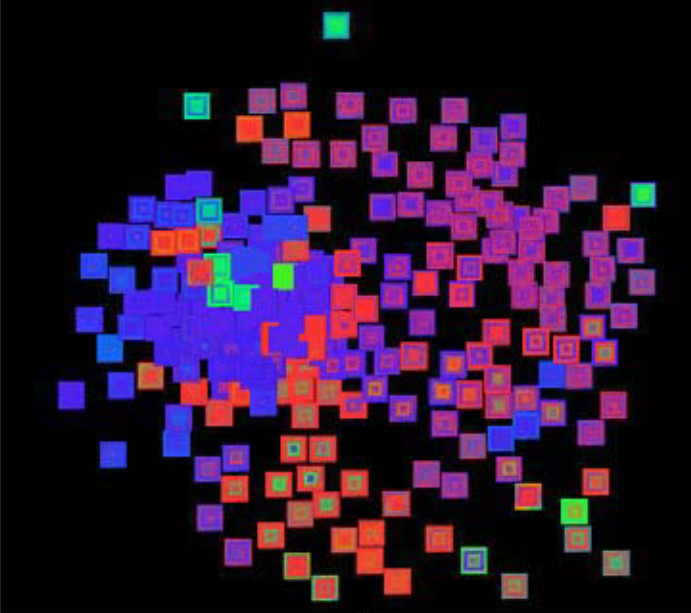
\includegraphics[width=\textwidth]{images/var1.png}
        \caption{}
        \label{fig:var1}
    \end{subfigure}%
    ~ %add desired spacing between images, e. g. ~, \quad, \qquad etc.
    \begin{subfigure}[b]{0.475\textwidth}
        \centering
        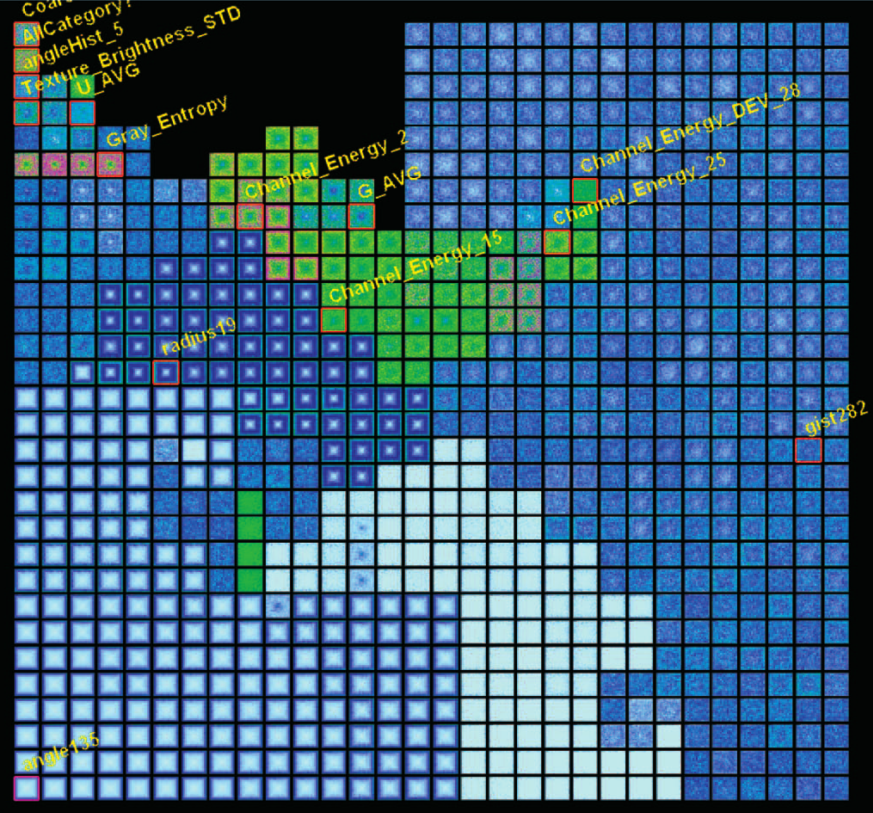
\includegraphics[width=\textwidth]{images/var2.png}
        \caption{}
        \label{fig:var2}
    \end{subfigure}
    \caption[VaR: Value and Relation]{asd}
    \label{fig:met}
\end{figure}


%--------------------------------------------------------------------------------
\subsection{Similaridade entre Dimensões}\label{ss:sim}

Uma tarefa fundamental para a execução deste trabalho é maneira como define-se a            similaridade entre as dimensões. Este problema pode ser formulado da seguinte maneira~\cite{Ankerst1998}: Dado um conjunto de dados contendo $n$ elementos com $m-$dimensões, suas colunas podem ser descritas por $m$ vetores $A_i~(0 \leq i < m)$, cada uma contendo $n$ números reais $a_{i,k}, (0 \leq k < n)$. Deseja-se definir uma medida de similaridade $S$ que dado dois vetores retorne um número real ($S : \mathbb{R}^n \times \mathbb{R}^n \rightarrow \mathbb{R}$) que satisfaça as seguintes propriedades:

\begin{enumerate}

    \item Positividade: $\forall A_i,A_j \in \mathbb{R}^n: S(A_i,A_j) \geq 0 $

    \item Reflexividade: $\forall A_i,A_j \in \mathbb{R}^n: (A_i = A_j) \Leftrightarrow S(A_i,A_j) = 0 $

    \item Simetria: $\forall A_i,A_j \in \mathbb{R}^n: S(A_i,A_j) = S(A_j,A_i)$, onde $(0 \leq i,j < d)$.

\end{enumerate}

Uma medida de similaridade entre duas variáveis $x$ e $y$ muito utilizada é o coeficiente de correlação linear de Pearson $p$, dado por:

\begin{equation}
    p(x,y) = \frac{cov(x,y)}{\sqrt{var(x)var(y)}},
\end{equation}

\noindent onde $var$ corresponde à variância e $cov$ à covariância. Quando $x$ e $y$ são completamente dependentes entre si, o valor de $p(x,y)$ é $1$ ou $-1$. Caso não exista nenhuma dependência linear entre as variáveis, o valor obtido é $0$. Porém, nos conjuntos de dados as relações entre as variáveis nem sempre são lineares e daí que surge a maior limitação deste coeficiente. Como pode ser observado pela Figura~\ref{fig:corrs} e pelos valores apresentados na Tabela~\ref{tab:corrs}, a medida não é capaz de capturar dependências não lineares entre as variáveis. 

\begin{figure}[h!]
    \centering
    \begin{subfigure}[b]{0.5\textwidth}
        \centering
        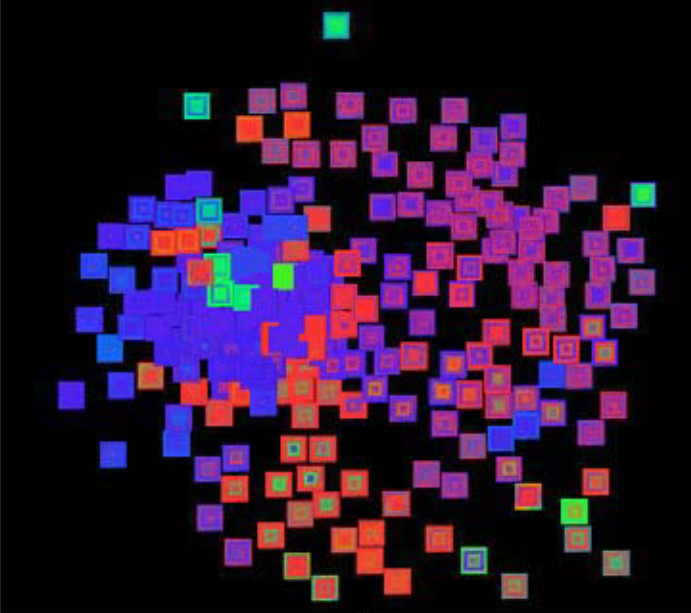
\includegraphics[width=\textwidth]{images/var1.png}
        \caption{}
        \label{fig:var1}
    \end{subfigure}%
    ~ %add desired spacing between images, e. g. ~, \quad, \qquad etc.
    \begin{subfigure}[b]{0.475\textwidth}
        \centering
        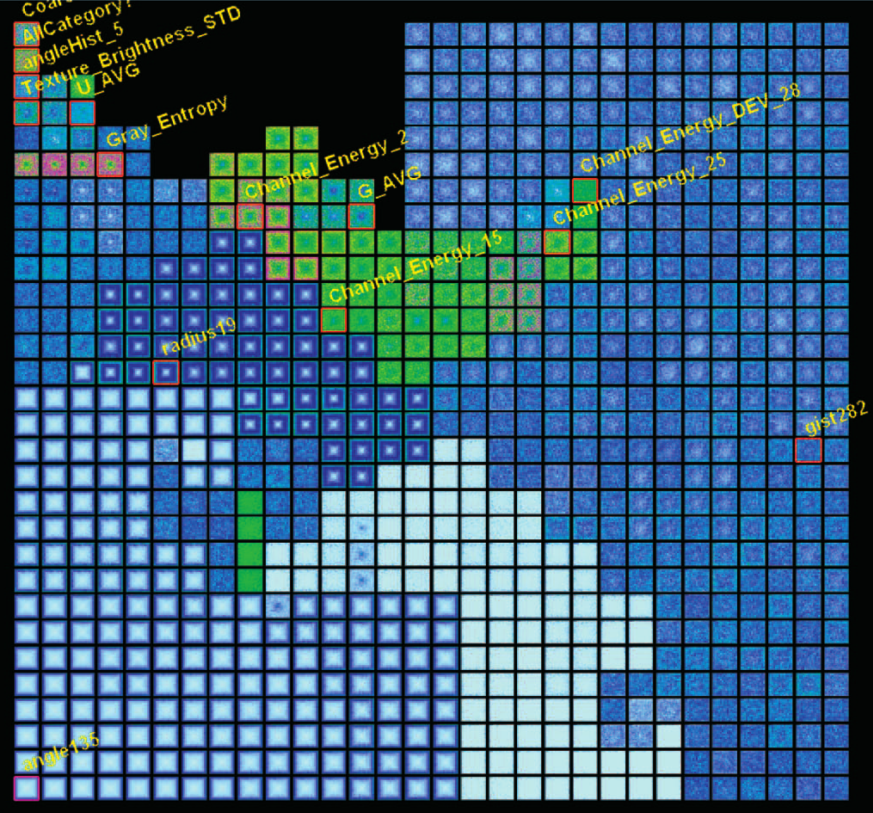
\includegraphics[width=\textwidth]{images/var2.png}
        \caption{}
        \label{fig:var2}
    \end{subfigure}
    \caption[VaR: Value and Relation]{asd}
    \label{fig:corrs}
\end{figure}

\begin{table}
    \caption[Cronograma de atividades]{Cronograma de Atividades. As marcações em preto        indicam atividades que são priorizadas no período.}
    \begin{center}
        \begin{tabular}{|c|c|c|c|c|c|c|}
        \end{tabular}
    \end{center}
    \label{tab:corrs}
\end{table}

% Introduzo MI (ler Kraskov) 

% Descrevo um estimador de MI, outros estimadores de MI: 12,13,14

% Apresento o problema de MI e MIC como a solução (apresentar complexidade computacional da MIC)

Na literatura encontram-se diversos outros métodos que poderiam ser utilizados para o cálculo de similaridade. Métodos de regressão~\cite{Friedman2001, Cleveland1988, Stone1977} têm bom desempenho quando as relações podem ser descritas por uma função, mas além desta situação falham em encontrar até os mais simples relacionamentos. Os métodos baseados em curvas principais~\cite{Hastie1989, Tibshirani1992, Delicado2008} e outros de correlação~\cite{Reny1959, Breiman1985, Kosorok2009} são aplicáveis a um domínio mais abrangente de dados, porém não conseguem capturar os relacionamentos tão eficientemente quanto a medida MIC~\cite{Reshef2011} mesmo para casos simples, como pode ser observado pela Tabela~\ref{tab:corrs}.    

A qualidade de uma medida de similaridade costuma variar de acordo com o domínio em que é aplicada. Normalmente, uma medida é dita adequada quando há uma concordância entre o valor obtido e a opinião de um especialista da área. No entanto, mesmo um especialista sobre um assunto pode ter dificuldade em determinar com precisão a semelhança entre dois objetos. Assim, é muito difícil definir um modelo matemático que meça a similaridade entre dois atributos com precisão para todas as aplicações de forma genérica. A MIC é uma medida que se propõe a executar esta difícil tarefa e por isso foi escolhida como a medida de similaridade entre dimensões a ser utilizada neste trabalho. 


%--------------------------------------------------------------------------------
\subsection{Mapeamento no Espaço Bidimensional}

O mapeamento dos elementos em um espaço bidimensional se baseia em algum método de redução de dimensionalidade. 

Um ponto fundamental para o mapeamento dos elementos no plano é compreender o erro embutido no processo. O resultado ótimo de qualquer método de redução é levar os dados de m em p, onde p equivale à dimensionalidade intrínseca dos dados. No entanto,  não há garantias de que p equivale à um espaço bidimensional, assim ao mapear os dados em um plano, a dimensionalidade dos dados será reduzida além da dimensionalidade intrínseca e consequentemente haverá perda de informação.

Conclui-se que independentemente do método de redução adotado, a não ser que a dimensionalidade intrínseca dos dados seja equivalente a dois, haverá um erro ao mapear os dados em um plano. Dois tipos de erros podem ocorrer: pontos similares posicionados distantes entre si (falsos negativos), ou pontos diferentes posicionados próximos entre si (falsos positivos). 

Em uma analogia à tarefa de recuperação de informação \emph{information retrieval}, esses erros podem ser associados respectivamente às medidas de precisão \emph{precision} e revocação \emph{recall} (citar 8 e 9 de Kaski).

% Tenho que falar do erro embutido 
Uma vez definido o cálculo de similaridade entre as dimensões, cria-se uma matriz de distâncias 

Não é possível ter garantias de que a dimensionalidade intrínseca dos dados se encaixa no plano bi
Ao mapear os dados em um plano bidimensional não é possível garantir que a dimensionalidade  

\subsection{Projeção das Dimensões}

\subsection{Projeção dos Itens}

O propósito principal da visualização da projeção dos itens é possibilitar que o usuário crie subconjuntos dos dados, por exemplo, possibilitar a remoção de \emph{outliers} ou a inspeção de um grupo de interesse.

Além disso esta visualização serve como um ferramenta adicional aos resultados dos classificadores para avaliar a separação entre os itens.


%--------------------------------------------------------------------------------
\subsection{Mecanismos de Interação}


%--------------------------------------------------------------------------------
\subsection{Forma de Avaliação}

% Tenho que falar aqui que vou aplicar diferentes métodos de redução (eventualmente ter que explicar os que eu escolhi cada um, de preferência falar que cada um tem uma característica específica) e em seguida vou verificar a qualidade da classificação e o tempo de execução do classificador.

A forma mais adotada na literatura para a avaliação de métodos de redução de dimensionalidade é a comparação dos erros obtidos em tarefas de classificação ao utilizar diferentes técnicas. 

Ao reduzir o número de atributos irrelevantes ou redundantes, pode-se melhorar o desempenho computacional e a precisão das técnicas operando sobre os dados, como agrupadores e classificadores de dados. Pretende-se avaliar as contribuições deste trabalho justamente pela quantificação do desempenho de tais métodos ao utilizar as técnicas desenvolvidas, seguida de uma comparação com técnicas já estabelecidas na literatura.

% O popular método K-Means será utilizado neste trabalho para se avaliar Para se avaliar o resultado obtido por agrupadores de dados, frequentemente utiliza-se a medida da silhueta e o índice I. A silhueta mede a .... O índice I é utilizado para...

% Falo de SVM-Precisão, Recall (FN?) e sei la o que...


%--------------------------------------------------------------------------------
\section{Resultados Esperados}

%--------------------------------------------------------------------------------
\section{Resultados Preliminares}

%--------------------------------------------------------------------------------
\section{Plano de Atividades e Cronograma Previsto}\label{sec:cronograma}

As principais atividades deste trabalho de mestrado são as seguintes:

\begin{enumerate}

    \item Cumprimento dos créditos das disciplinas exigidos pelo programa;

    \item Exame de proficiência em língua inglesa;

    \item Levantamento bibliográfico sobre técnicas de visualização computacional e redução de dimensionalidade;   

    \item Levantamento bibliográfico sobre técnicas visuais interativas para redução de dimensionalidade;  

    \item Adoção e implementação de uma metodologia para o cálculo da similaridade entre dimensões;

    \item Escrita da monografia de qualificação e sua apresentação para uma banca avaliadora;

    \item Implementação de um modelo visual que transmita simultaneamente informações sobre os itens e dimensões de uma base de dados;

    \item Desenvolvimento de mecanismos de seleção e combinação para redução interativa de dimensionalidade;

    \item Desenvolvimento de um mecanismo interativo para transformação do espaço de atributos;

    \item Avaliação dos Resultados;

    \item Redação de artigos científicos e participação em congressos e eventos; 

    \item Escrita da dissertação de mestrado bem como sua apresentação para uma banca avaliadora;

\end{enumerate}

O cronograma de execução das atividades é apresentado na Tabela~\ref{t:atividades}, assumindo um projeto de duração de vinte e quatro meses.

\newcommand{\y}{\color{black}\rule{20pt}{7pt}}
\newcommand{\x}{\hspace*{20pt}}
\renewcommand{\r}{\color{cinza}\rule{20pt}{7pt}}

\setlength{\tabcolsep}{0pt}

\begin{table} 
    \caption[Cronograma de atividades]{Cronograma de Atividades. As marcações em preto indicam atividades que são priorizadas no período.}
    \begin{center}
        \begin{tabular}{|c|c|c|c|c|c|c|}
            \cline{2-7}
            \multicolumn{1}{l|}{} & \multicolumn{2}{c|}{2012} & \multicolumn{2}{c|}{2013} &        \multicolumn{2}{c|}{2014} \\
            \hline \ Atividade\ \ 
            & 1\textordmasculine\ S. & 2\textordmasculine\ S. 
            & 1\textordmasculine\ S. & 2\textordmasculine\ S. 
            & 1\textordmasculine\ S. & 2\textordmasculine\ S. \\
            \hline \hline                                        
            %     &       2012        &       2013         &       2014       \\
            1     &\y\y    &\y\y      &\x\x     &\x\x      &\x\x     &\x\x    \\ \hline
            2     &\x\y    &\x\x      &\x\x     &\x\x      &\x\x     &\x\x    \\ \hline
            3     &\x\x    &\y\y      &\y\y     &\r\r      &\r\r     &\x\x    \\ \hline
            4     &\x\x    &\y\y      &\y\y     &\r\r      &\r\r     &\x\x    \\ \hline
            5     &\x\x    &\x\x      &\y\y     &\x\x      &\x\x     &\x\x    \\ \hline
            6     &\x\x    &\x\x      &\y\y     &\x\x      &\x\x     &\x\x    \\ \hline
            7     &\x\x    &\x\x      &\x\y     &\r\x      &\x\x     &\x\x    \\ \hline
            8     &\x\x    &\x\x      &\x\x     &\r\r      &\x\x     &\x\x    \\ \hline
            9     &\x\x    &\x\x      &\x\x     &\r\r      &\x\x     &\x\x    \\ \hline
            10     &\x\x    &\x\x      &\x\x     &\x\r      &\r\r     &\x\x    \\ \hline
            11     &\x\x    &\x\y      &\y\y     &\r\r      &\r\r     &\x\x    \\ \hline
            12     &\x\x    &\x\x      &\x\x     &\x\r      &\r\r     &\x\x    \\ \hline
            %     &       2012        &       2013         &       2014       \\
        \end{tabular}
    \end{center}
    \label{t:atividades}
\end{table}
